\documentclass{standalone}
\usepackage{graphicx}	
\usepackage{amssymb, amsmath, amsthm}
\usepackage{color}

\usepackage{tikz}
\usetikzlibrary{intersections, backgrounds}

\definecolor{light}{RGB}{220, 188, 188}
\definecolor{mid}{RGB}{185, 124, 124}
\definecolor{dark}{RGB}{143, 39, 39}
\definecolor{highlight}{RGB}{180, 31, 180}
\definecolor{gray10}{gray}{0.1}
\definecolor{gray20}{gray}{0.2}
\definecolor{gray30}{gray}{0.3}
\definecolor{gray40}{gray}{0.4}
\definecolor{gray60}{gray}{0.6}
\definecolor{gray70}{gray}{0.7}
\definecolor{gray80}{gray}{0.8}
\definecolor{gray90}{gray}{0.9}
\definecolor{gray95}{gray}{0.95}

\begin{document}

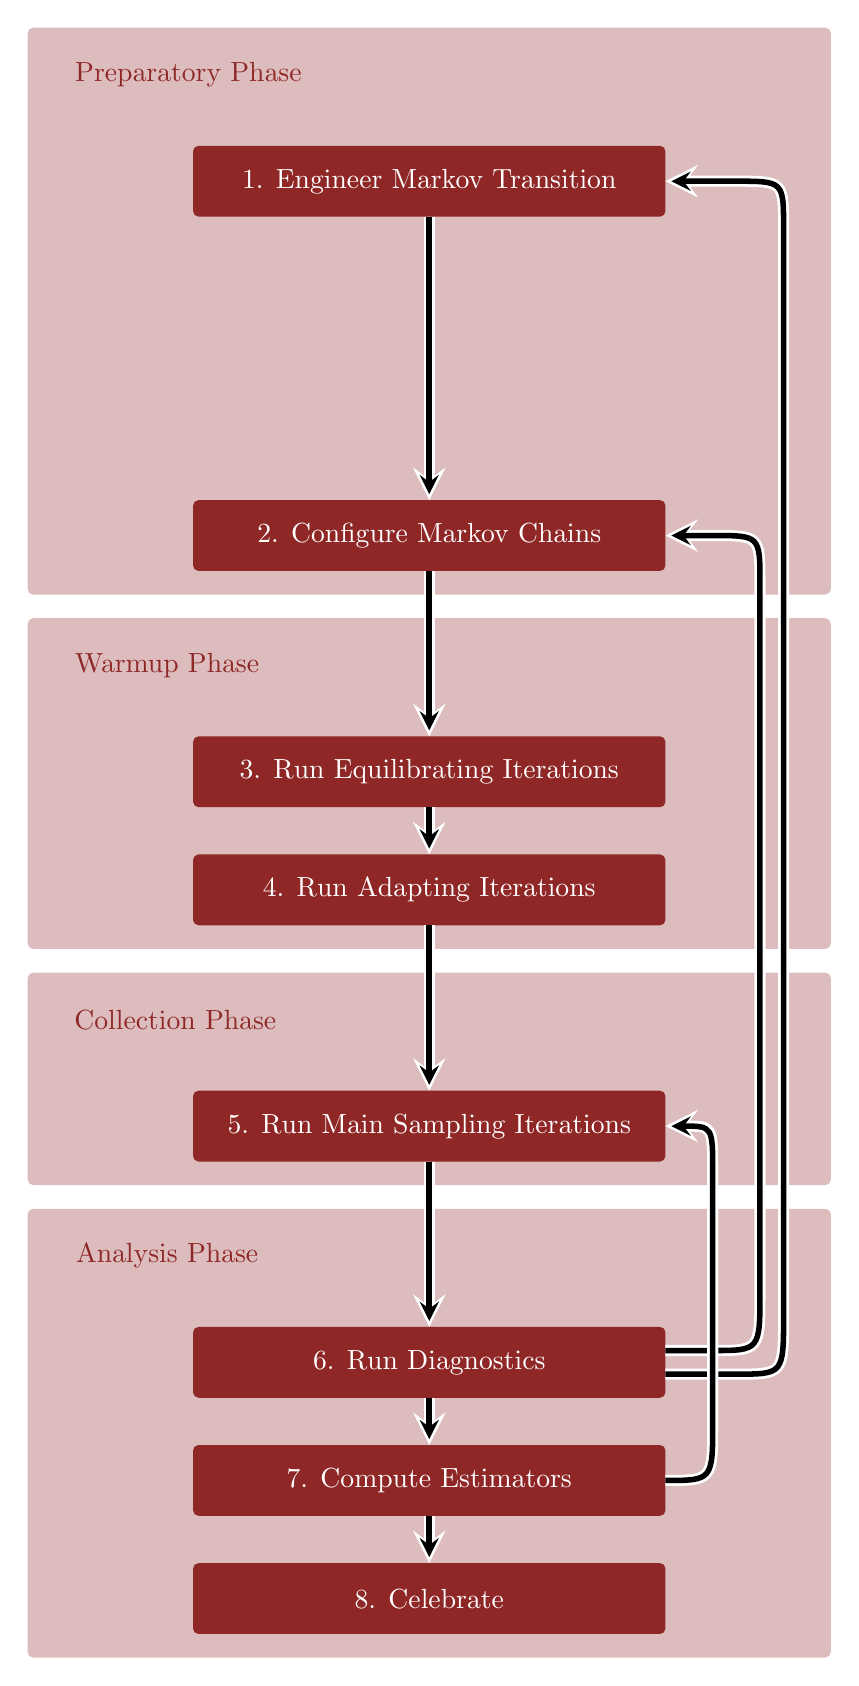
\begin{tikzpicture}[scale=0.3, thick]

  % Configuration
  \fill [rounded corners=2pt, light] (-7, 44) rectangle (27, 68);
  \node[align=left, dark] at (0, 66) { Preparatory Phase };
  
  % Warmup
  \fill [rounded corners=2pt, light] (-7, 29) rectangle (27, 43);
  \node[align=center, dark] at (-1.1, 41) { Warmup Phase};

  % Collection
  \fill [rounded corners=2pt, light] (-7, 19) rectangle (27, 28);
  \node[align=center, dark] at (-0.75, 26) { Collection Phase};
 
  % Analysis
  \fill [rounded corners=2pt, light] (-7, -1) rectangle (27, 18);
  \node[align=center, dark] at (-0.9, 16) { Analysis Phase };
  
  %\draw[blue] (-5, 63) -- (-5, 0);

  % Step One
  \fill [rounded corners=2pt, fill=dark, text=white] (0, 60) rectangle +(20, 3) 
  node [midway, align=center] {1. Engineer Markov Transition};
  
  \draw [->, >=stealth, white, line width=4] (10, 60) -- (10, 48);
  \draw [->, >=stealth, line width=2] (10, 60) -- (10, 48.25);

  % Step Three
  \fill [rounded corners=2pt, fill=dark, text=white] (0, 45) rectangle +(20, 3) 
  node [midway, align=center] {2. Configure Markov Chains};
  
  \draw [->, >=stealth, white, line width=4] (10, 45) -- (10, 38);
  \draw [->, >=stealth, line width=2] (10, 45) -- (10, 38.25);
  
  % Step Four
  \fill [rounded corners=2pt, fill=dark, text=white] (0, 35) rectangle +(20, 3) 
  node [midway, align=center] {3. Run Equilibrating Iterations};
  
  \draw [->, >=stealth, white, line width=4] (10, 35) -- (10, 33);
  \draw [->, >=stealth, line width=2] (10, 35) -- (10, 33.25);
  
  % Step Five
  \fill [rounded corners=2pt, fill=dark, text=white] (0, 30) rectangle +(20, 3) 
  node [midway, align=center] {4. Run Adapting Iterations};
  
  \draw [->, >=stealth, white, line width=4] (10, 30) -- (10, 23);
  \draw [->, >=stealth, line width=2] (10, 30) -- (10, 23.25);
  
  % Step Six
  \fill [rounded corners=2pt, fill=dark, text=white] (0, 20) rectangle +(20, 3) 
  node [midway, align=center] {5. Run Main Sampling Iterations};
  
  \draw [->, >=stealth, white, line width=4] (10, 20) -- (10, 13);
  \draw [->, >=stealth, line width=2] (10, 20) -- (10, 13.25);

  % Step Seven
  \fill [rounded corners=2pt, fill=dark, text=white] (0, 10) rectangle +(20, 3) 
  node [midway, align=center] {6. Run Diagnostics};
  
  \draw [->, >=stealth, white, line width=4] (10, 10) -- (10, 8);
  \draw [->, >=stealth, line width=2] (10, 10) -- (10, 8.25);

  \draw [->, >=stealth, white, line width=4] 
    (20, 12) -- (22, 12) .. controls (24, 12) .. (24, 14.5) -- 
    (24, 44.5) .. controls (24, 46.5) .. (22, 46.5) -- (20, 46.5);

  \draw [->, >=stealth, line width=2] 
    (20, 12) -- (22, 12) .. controls (24, 12) .. (24, 14.5) -- 
    (24, 44.5) .. controls (24, 46.5) .. (22, 46.5) -- (20 + 0.25, 46.5);

  \draw [->, >=stealth, white, line width=4] 
    (20, 11) -- (23, 11) .. controls (25, 11) .. (25, 13.5) -- 
    (25, 59.5) .. controls (25, 61.5) .. (23, 61.5) -- (20, 61.5);

  \draw [->, >=stealth, line width=2] 
    (20, 11) -- (23, 11) .. controls (25, 11) .. (25, 13.5) -- 
    (25, 59.5) .. controls (25, 61.5) .. (23, 61.5) -- (20 + 0.25, 61.5);
  
  % Step Eight
  \fill [rounded corners=2pt, fill=dark, text=white] (0, 5) rectangle +(20, 3) 
  node [midway, align=center] {7. Compute Estimators};

  \draw [->, >=stealth, white, line width=4] (10, 5) -- (10, 3);
  \draw [->, >=stealth, line width=2] (10, 5) -- (10, 3.25);

  \draw [->, >=stealth, white, line width=4] 
    (20, 6.5) .. controls (22, 6.5) .. (22, 9) -- 
    (22, 19.5) .. controls (22, 21.5) .. (20, 21.5);

  \draw [->, >=stealth, line width=2] 
    (20, 6.5) .. controls (22, 6.5) .. (22, 9) -- 
    (22, 19.5) .. controls (22, 21.5) .. (20.25, 21.5);

  % Step Nine
  \fill [rounded corners=2pt, fill=dark, text=white] (0, 0) rectangle +(20, 3) 
  node [midway, align=center] {8. Celebrate};
  
\end{tikzpicture}

\end{document}  